\documentclass[10pt,twocolumn]{article}

\usepackage[utf8]{inputenc}
\usepackage[english]{babel}
\usepackage{amsmath,amssymb}
\usepackage[margin=1.5cm,top=2cm,bottom=2cm]{geometry}
\usepackage{caption}
\captionsetup{labelfont={bf},font=small,skip=4pt}
\usepackage{cite}
\usepackage{color}
\usepackage{fancyhdr}
\pagestyle{fancy}
\fancyhf{}
\fancyhead[L]{\footnotesize IST}
\fancyhead[R]{\footnotesize ULisboa}
\fancyfoot[L]{\footnotesize SCDTR 2025/2026}
\fancyfoot[C]{\thepage}
\fancyfoot[R]{\footnotesize MEE}
\renewcommand{\footrulewidth}{0.4pt}
\usepackage{float}
\usepackage{graphicx}
\usepackage[colorlinks=true,linkcolor=istblue,urlcolor=istblue,citecolor=istblue]{hyperref}
\usepackage{indentfirst}
\usepackage{siunitx}
\usepackage{subcaption}
\usepackage{booktabs}
\usepackage{titlesec}
\titleformat{\section}{\normalsize\bfseries}{\thesection}{0.6em}{}
\titleformat{\subsection}{\small\bfseries}{\thesubsection}{0.6em}{}
\titlespacing{\section}{0pt}{8pt}{3pt}
\titlespacing{\subsection}{0pt}{5pt}{2pt}
\usepackage{enumitem}
\setlist{nosep,leftmargin=*}
\setlength{\parskip}{2pt}
\setlength{\parindent}{0.6em}
\setlength{\columnsep}{0.6cm}
\usepackage[european,siunitx]{circuitikz}

\newcommand{\HRule}{\rule{\linewidth}{0.5mm}}
\definecolor{istblue}{RGB}{3, 171, 230}

\begin{document}

% --- Cover ---
\twocolumn[{%
\begin{center}
\vspace{0.5cm}
\includegraphics[scale=0.25]{IST_logo.png}\\[0.5cm]
\textsc{\Large Distributed Real-Time Control Systems}\\[0.4cm]
\textsc{\large Master's in Electrical and Computer Engineering}\\[0.6cm]
\HRule\\[0.2cm]
{\normalsize \bf Mid-Term Report --- Local Luminaire Controller}\\[0.1cm]
\HRule\\[0.4cm]
\begin{minipage}{0.45\textwidth}
\begin{flushleft}\small Jo\~{a}o Rocha (IST1106509)\end{flushleft}
\end{minipage}%
\begin{minipage}{0.45\textwidth}
\begin{flushright}\small\href{mailto:joao.s.rocha@tecnico.ulisboa.pt}{\texttt{joao.s.rocha@tecnico.ulisboa.pt}}\end{flushright}
\end{minipage}\\[0.3cm]
{\large 2025/2026 -- Spring Semester}
\vspace{0.2cm}
\end{center}
}]

% ======================================================================
\section{Introduction}

This report presents the design, implementation and experimental validation of a local luminaire controller, constituting the first stage of a distributed illumination control system. The system is built around a Raspberry Pi Pico microcontroller and targets the regulation of desk-surface illuminance to configurable set-points under varying occupancy conditions. Each luminaire node comprises a white LED~\cite{led} driven by pulse-width modulation (PWM), a cadmium sulphide (CdS) light-dependent resistor (LDR)~\cite{ldr} serving as the illuminance sensor, and embedded firmware implementing a proportional-integral (PI) controller with anti-windup protection. The controller must track reference changes with a settling time below \SI{0.5}{\second} while maintaining near-zero overshoot, low flicker, and minimal steady-state error.

\section{Hardware Assembly}

The luminaire was assembled inside a white-lined cardboard box (Fig.~\ref{fig:box}). The LED is driven from GP15 through a \SI{47}{\ohm} current-limiting resistor at \SI{30}{\kilo\hertz} PWM with 12-bit resolution (0--4095). The LDR sensing circuit (Fig.~\ref{fig:circuit}) is a voltage divider formed by the LDR and a \SI{10}{\kilo\ohm} fixed resistor, with a \SI{10}{\micro\farad} electrolytic capacitor between the output node and ground. This RC network ($\tau_\mathrm{RC} \approx \SI{100}{\milli\second}$) attenuates PWM-coupled noise and smooths the inherent persistence transients of the CdS photoresistor. The 12-bit ADC reads the filtered output on pin A0.

\begin{figure}[H]
  \centering
  \begin{subfigure}[t]{0.48\columnwidth}
    \centering
    \fbox{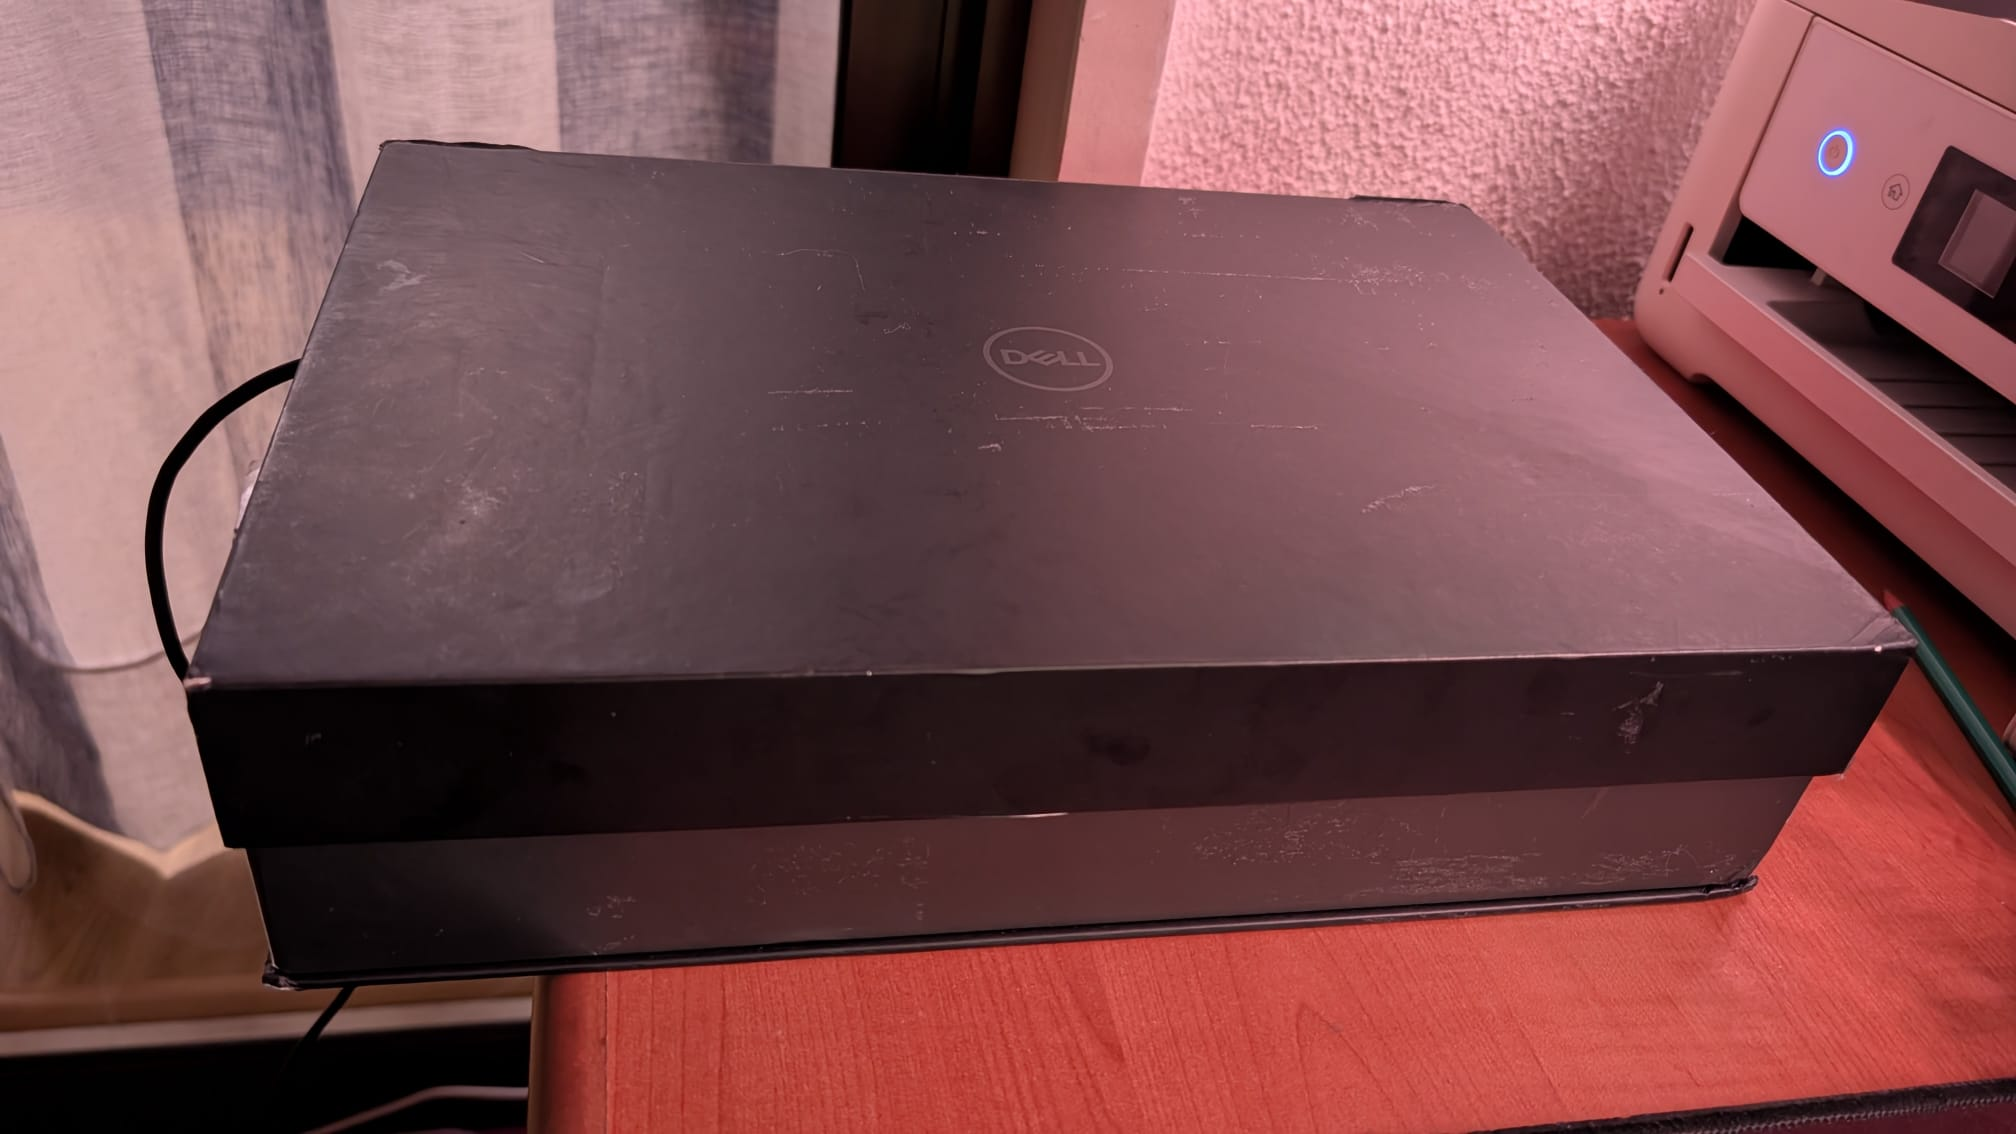
\includegraphics[width=\linewidth]{figures/box_exterior.jpeg}}
    \caption{Exterior.}
  \end{subfigure}
  \hfill
  \begin{subfigure}[t]{0.48\columnwidth}
    \centering
    \fbox{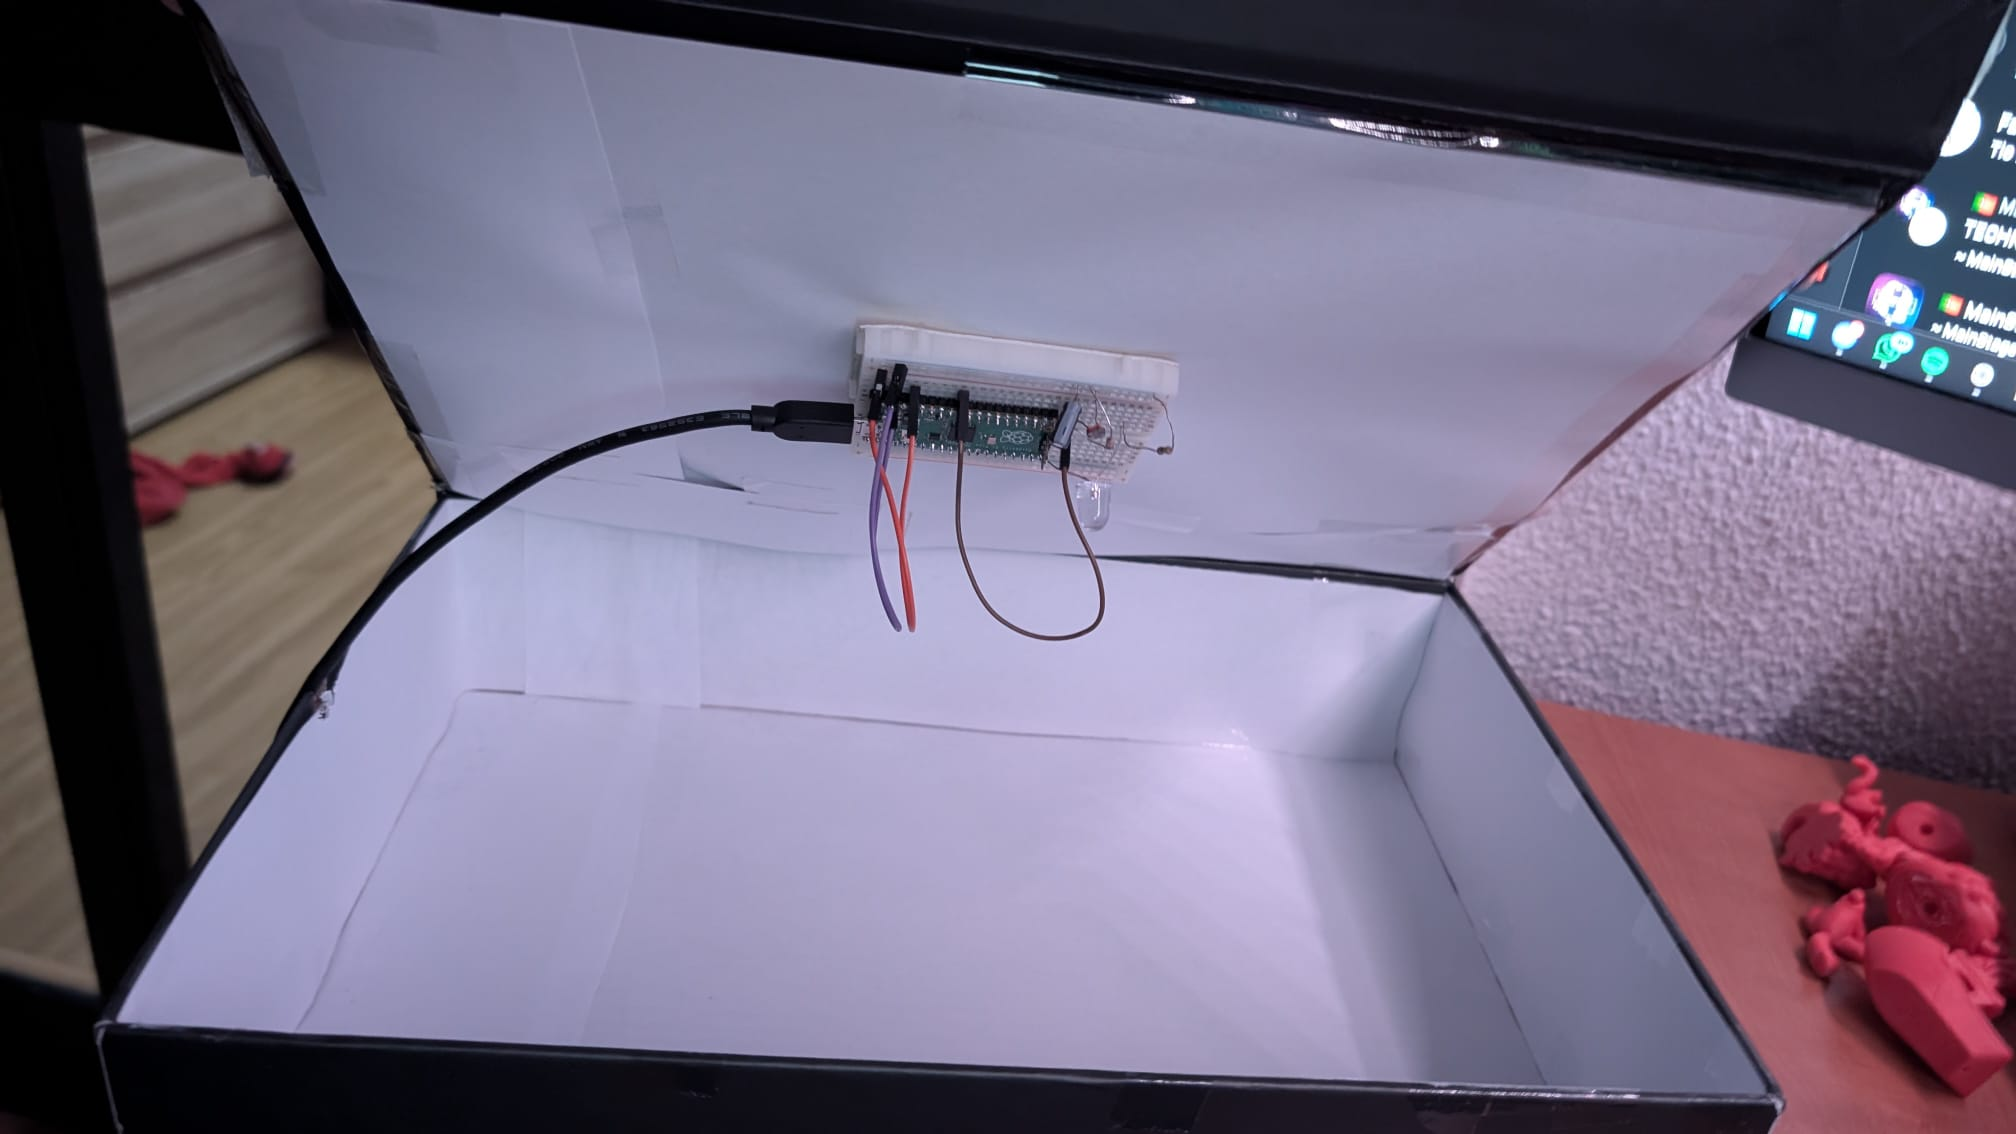
\includegraphics[width=\linewidth]{figures/box_interior.jpeg}}
    \caption{Interior.}
  \end{subfigure}
  \caption{Luminaire box model with LED and LDR mounted.}
  \label{fig:box}
\end{figure}

\begin{figure}[H]
  \centering
  \begin{circuitikz}[scale=0.75, transform shape, european]
    % LED driver (left side)
    \draw (0,4) node[above]{GP15}
      to[short] (1,4)
      to[R, l=\SI{47}{\ohm}] (3,4)
      to[led, l_=LED] (3,2)
      to[short] (3,1.5) node[ground]{};
    % LDR circuit (right side)
    \draw (5,4) node[above]{$V_\mathrm{cc}=\SI{3.3}{\volt}$}
      to[short] (5,3.5)
      to[vR, l=LDR] (5,1.5)
      to[short] (5,1) -- (7,1)
      to[R, l_=\SI{10}{\kilo\ohm}] (7,-1)
      node[ground]{};
    % Capacitor
    \draw (5,1) -- (5,0)
      to[C, l_=\SI{10}{\micro\farad}] (5,-1)
      node[ground]{};
    % ADC output
    \draw (5,1) to[short, -o] (8.5,1) node[right]{A0 (ADC)};
    % Voltage label
    \node at (6,1.3) {\footnotesize $v(t)$};
  \end{circuitikz}
  \caption{Circuit schematic: LED driver (left) and LDR sensing circuit with RC filter (right).}
  \label{fig:circuit}
\end{figure}

\section{Illuminance Measurement}

The CdS LDR resistance follows a log-log affine relationship with illuminance~\cite{projectguide}:
\begin{equation}
  \log_{10}(R_\mathrm{LDR}) = m \log_{10}(\mathrm{LUX}) + b
  \label{eq:ldr}
\end{equation}
which is inverted to obtain LUX from the measured ADC voltage via the voltage divider equation $R_\mathrm{LDR} = R_\mathrm{fixed}(V_\mathrm{cc}/V_\mathrm{out} - 1)$. The slope $m = -0.70$ was verified by sweeping the duty cycle inside the sealed box and confirming linearity of the LUX--duty relationship. The intercept $b = 5.847$ was calibrated against a known illuminance reference (\SI{500}{\lux} at \SI{1}{\metre} from laboratory fluorescent lighting).

Each measurement cycle acquires 100 rapid ADC samples (spanning $\sim$6 PWM periods) and averages them before the nonlinear log-log conversion. An exponential moving average (EMA) with $\alpha = 0.9$ ($\tau_\mathrm{EMA} \approx \SI{100}{\milli\second}$) provides additional software smoothing. The static gain $K_s$ and background illuminance $L_\mathrm{bg}$ are measured automatically at start-up via a calibration routine. All parameters are in Table~\ref{tab:params}.

\begin{table}[H]
\centering
\caption{Calibrated sensor and tuned controller parameters.}
\label{tab:params}
\small
\setlength{\tabcolsep}{4pt}
\begin{tabular}{@{}llll@{}}
  \toprule
  \multicolumn{2}{c}{\textbf{LDR Model}} & \multicolumn{2}{c}{\textbf{PI Controller}} \\
  \cmidrule(r){1-2}\cmidrule(l){3-4}
  $m = -0.70$        & log-log slope     & $K_p = 0.01$        & prop.\ gain \\
  $b = 5.847$        & log-log intercept & $K_i = 0.11$        & integ.\ gain \\
  $L_\mathrm{bg}=\SI{0.12}{\lux}$ & background & $b_\mathrm{sp}=1.0$ & SP weight \\
  $K_s=\SI{77}{\lux}$  & static gain    & $T_t=\SI{0.15}{\second}$ & AW time cst. \\
  $\alpha_\mathrm{EMA}=0.9$ & filter coeff. & Feedforward     & OFF \\
  \bottomrule
\end{tabular}
\end{table}

\section{Controller Design}

The controller is implemented as a C++ class evaluated at \SI{100}{\hertz}. A deliberate design decision was made to operate without feedforward. Although a feedforward term $u_\mathrm{ff} = (r - L_\mathrm{bg})/K_s$ can provide near-instantaneous open-loop response to reference changes, experimental testing revealed that the resulting abrupt duty-cycle transitions trigger the CdS LDR's persistence effect---a well-documented phenomenon in which the photoresistor's resistance continues to drift for 200--300\,ms after any sudden illumination change~\cite{ldr}. This persistence manifests as 30--40\% overshoot in the measured output (Fig.~\ref{fig:feedback}, red trace), regardless of the PI tuning. By disabling feedforward and relying exclusively on the PI controller, the duty cycle ramps gradually through the integrator action, and the LDR tracks the illuminance change smoothly without triggering persistence artefacts.

The discrete-time control law is:
\begin{equation}
  u[k] = K_p\bigl(b_\mathrm{sp}\,r[k] - y[k]\bigr) + I[k]
  \label{eq:pi}
\end{equation}
where $r[k]$ is the illuminance reference, $y[k]$ the measured illuminance, and $b_\mathrm{sp} = 1$ the set-point weight applied to the proportional term. The integral state incorporates back-calculation anti-windup:
\begin{equation}
  I[k] = I[k\!-\!1] + K_i\,T\,(r[k]\!-\!y[k]) + \frac{T}{T_t}\bigl(u_\mathrm{sat}[k\!-\!1]\!-\!u[k\!-\!1]\bigr)
  \label{eq:aw}
\end{equation}
When the output from~\eqref{eq:pi} exceeds the actuator limits $[0, 1]$, it is clipped to $u_\mathrm{sat}[k]$, and the last term in~\eqref{eq:aw} slowly discharges the accumulated integral error with a tracking time constant $T_t = \SI{0.15}{\second}$, preventing integrator windup. Bumpless transfer logic adjusts the integral state whenever gains are modified at run-time.

\section{Experimental Results}

\subsection{Step Response}

Fig.~\ref{fig:step} shows the controller tracking between $r_\mathrm{HIGH} = \SI{40}{\lux}$ and $r_\mathrm{LOW} = \SI{10}{\lux}$ with 6-second holds per phase. The HIGH$\to$LOW transition settles within approximately \SI{0.43}{\second} and the LOW$\to$HIGH transition within \SI{0.27}{\second}, both well under the \SI{0.5}{\second} target. The overshoot is less than 2.5\% (peak \SI{40.7}{\lux} vs.\ target \SI{40}{\lux}), and the steady-state error is below \SI{0.1}{\lux}.

\begin{figure}[H]
  \centering
  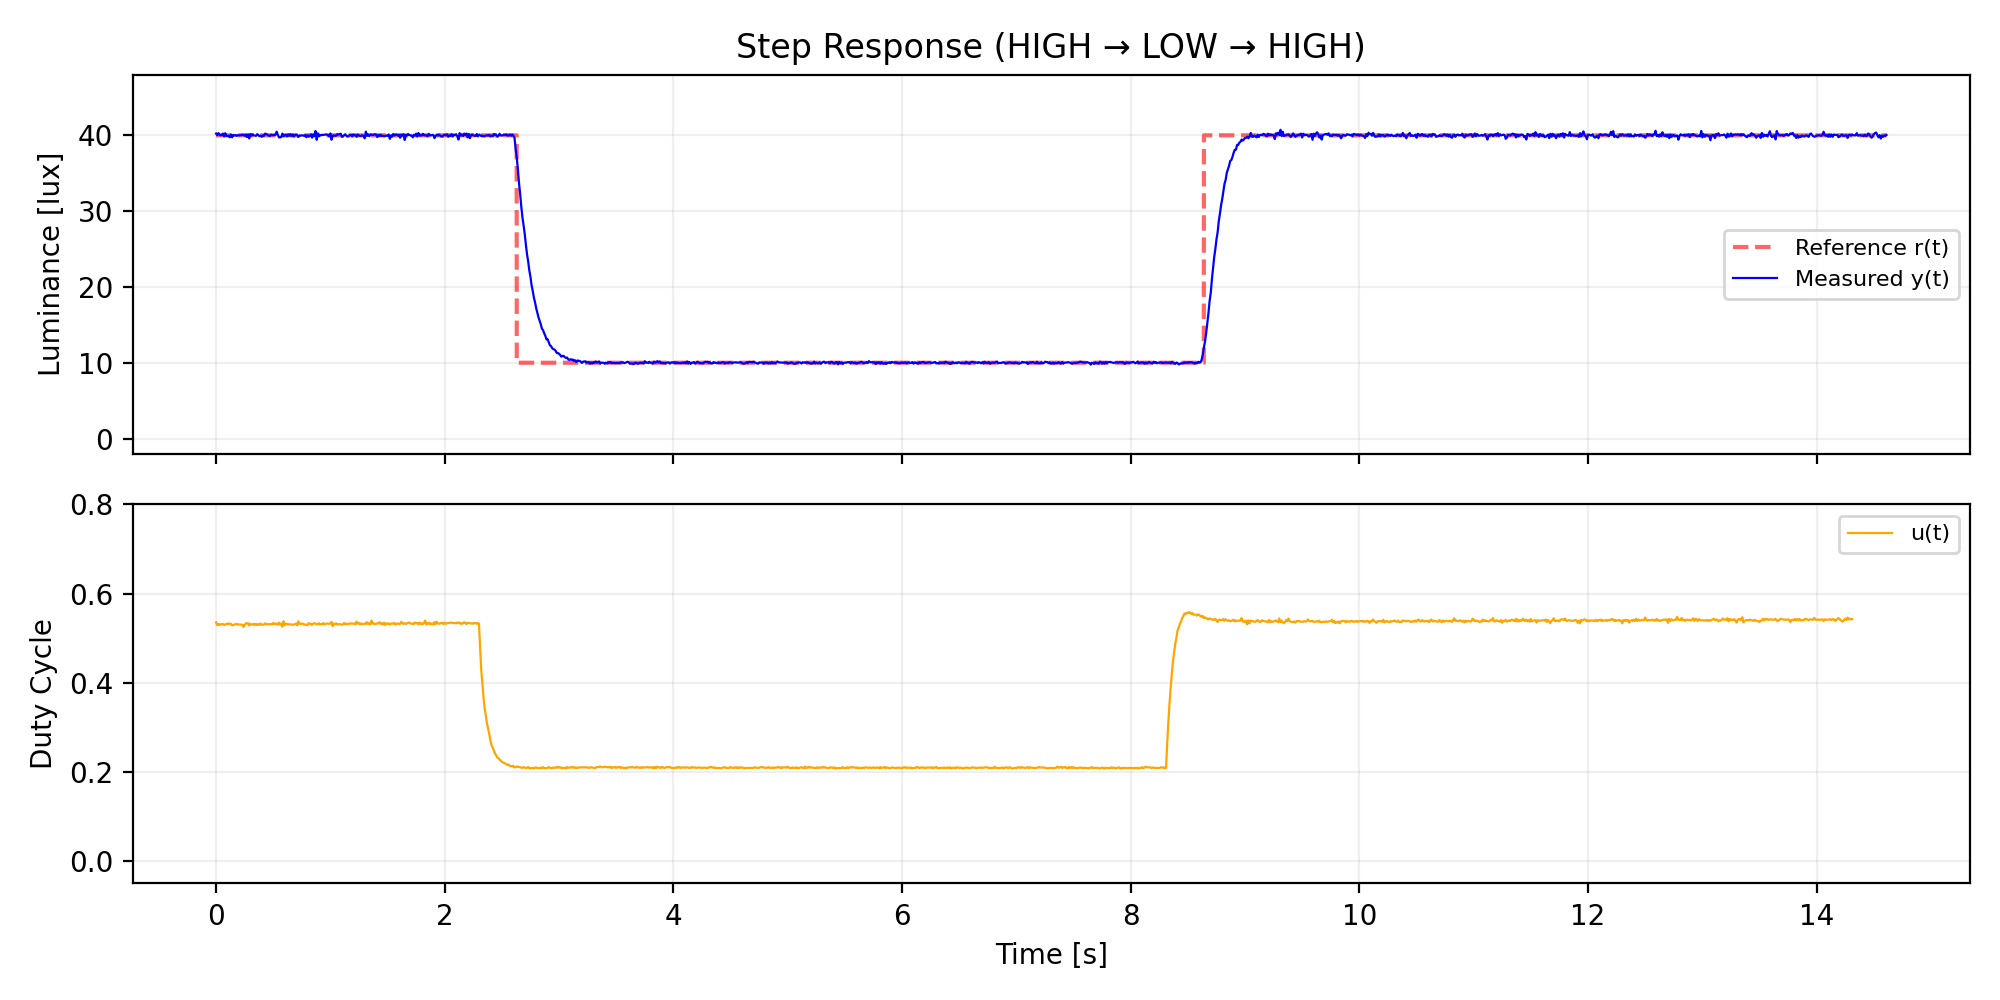
\includegraphics[width=\columnwidth]{figures/fig_step.png}
  \caption{Step response (HIGH$\to$LOW$\to$HIGH). Settling $<\SI{0.5}{\second}$, overshoot $<2.5\%$.}
  \label{fig:step}
\end{figure}

\subsection{Feedback vs.\ Feedforward Only}

Fig.~\ref{fig:feedback} compares PI feedback against a feedforward-only configuration where the duty cycle is set open-loop to $u = (r - L_\mathrm{bg})/K_s$. Without the PI loop, the HIGH reference produces only \SI{31}{\lux} (error $>\SI{9}{\lux}$) due to the mismatch between the linear gain model and the nonlinear LDR characteristic. The PI controller eliminates this error, demonstrating that feedback is essential even with a reasonably accurate plant model.

\begin{figure}[H]
  \centering
  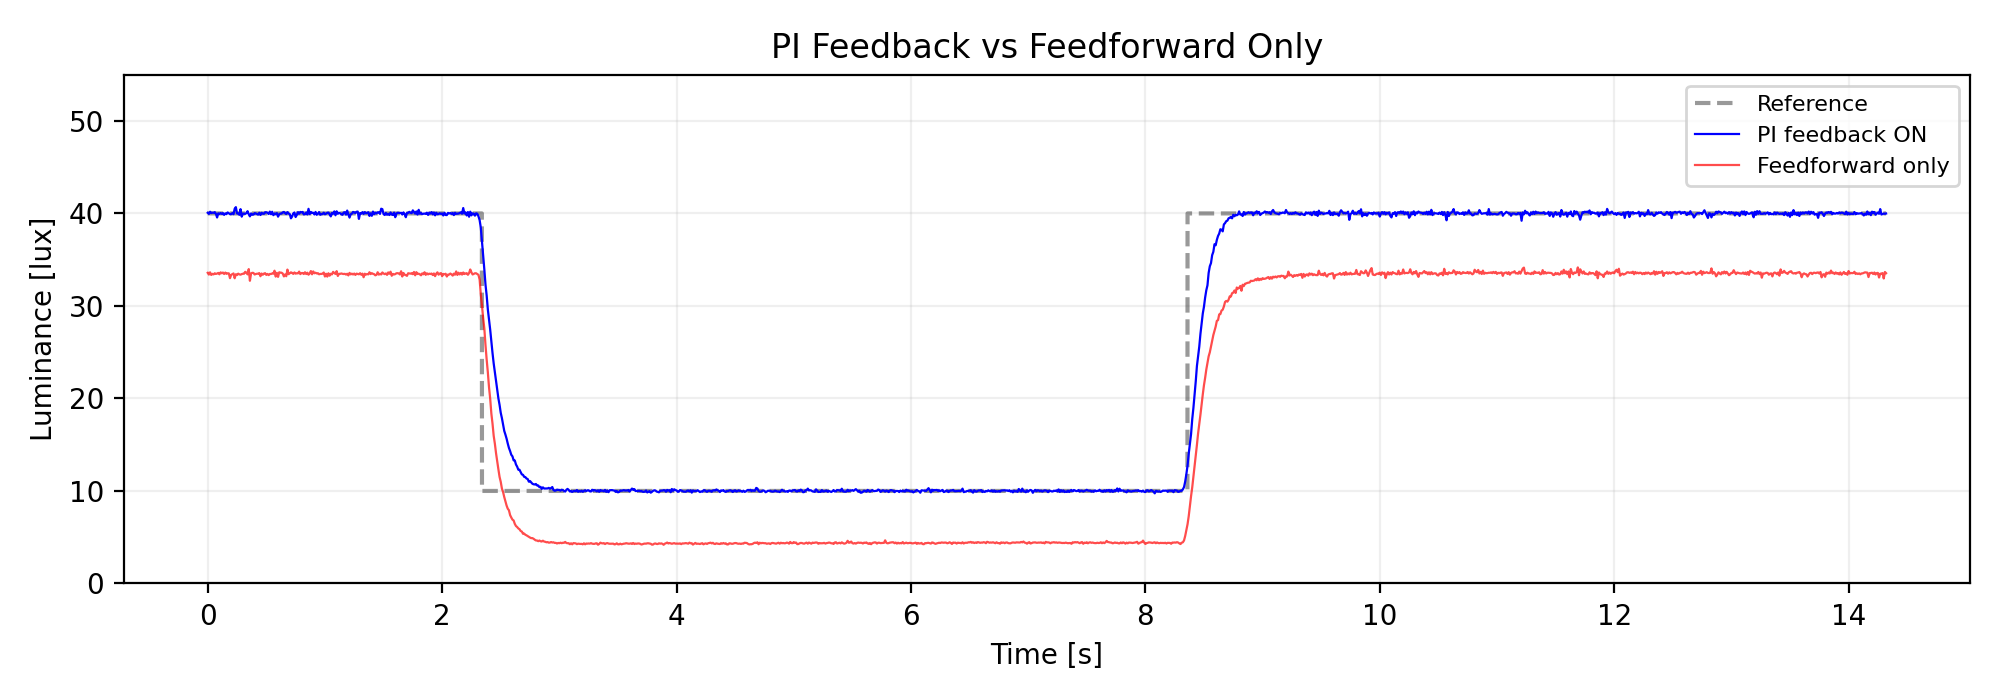
\includegraphics[width=\columnwidth]{figures/fig_feedback.png}
  \caption{PI feedback (blue) vs.\ feedforward only (red).}
  \label{fig:feedback}
\end{figure}

\subsection{Anti-Windup Evaluation}

Fig.~\ref{fig:antiwindup} compares the response with anti-windup ON and OFF. The traces nearly overlap because the PI-only architecture (without feedforward) produces moderate control signals that remain within the $[0, 1]$ saturation limits during normal transitions. The mechanism remains important as a safety net for extreme references or large disturbances where saturation would otherwise occur.

\begin{figure}[H]
  \centering
  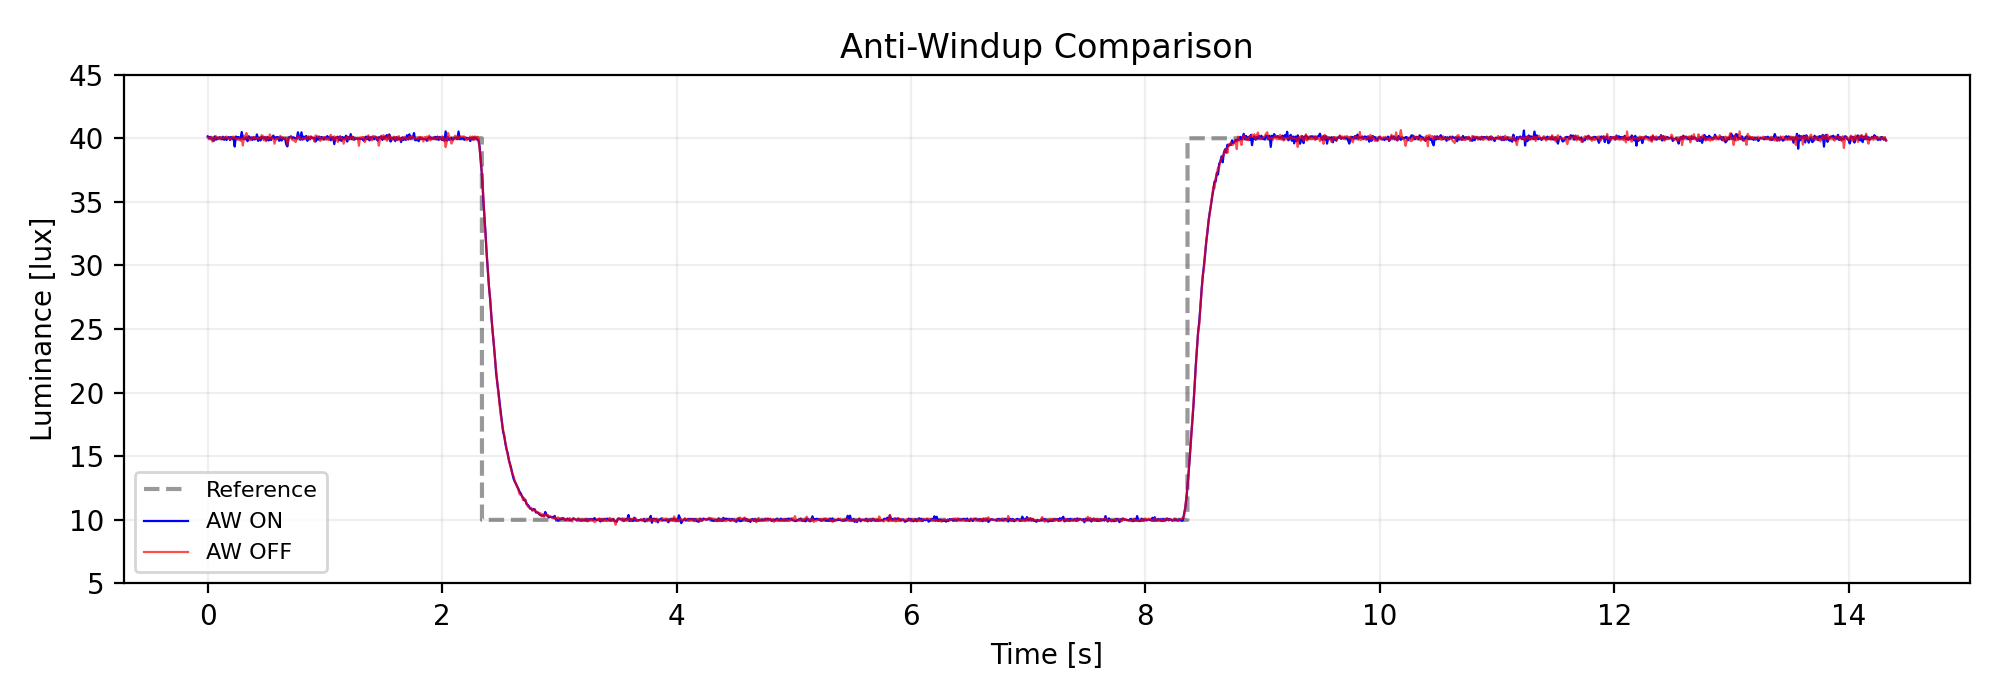
\includegraphics[width=\columnwidth]{figures/fig_antiwindup.png}
  \caption{Anti-windup ON (blue) vs.\ OFF (red).}
  \label{fig:antiwindup}
\end{figure}

\subsection{Disturbance Rejection}

Fig.~\ref{fig:disturbance} shows the response when the box lid was briefly opened at steady state. Opening the lid admits external light into the box, causing the measured illuminance to spike to \SI{48}{\lux}; the controller responds by reducing the duty from 0.58 to 0.40. When the lid is closed, the external light is removed and the illuminance dips to \SI{32}{\lux} before the controller ramps the duty back up. The system recovers to within 2\% of the reference in approximately \SI{2}{\second}.

\begin{figure}[H]
  \centering
  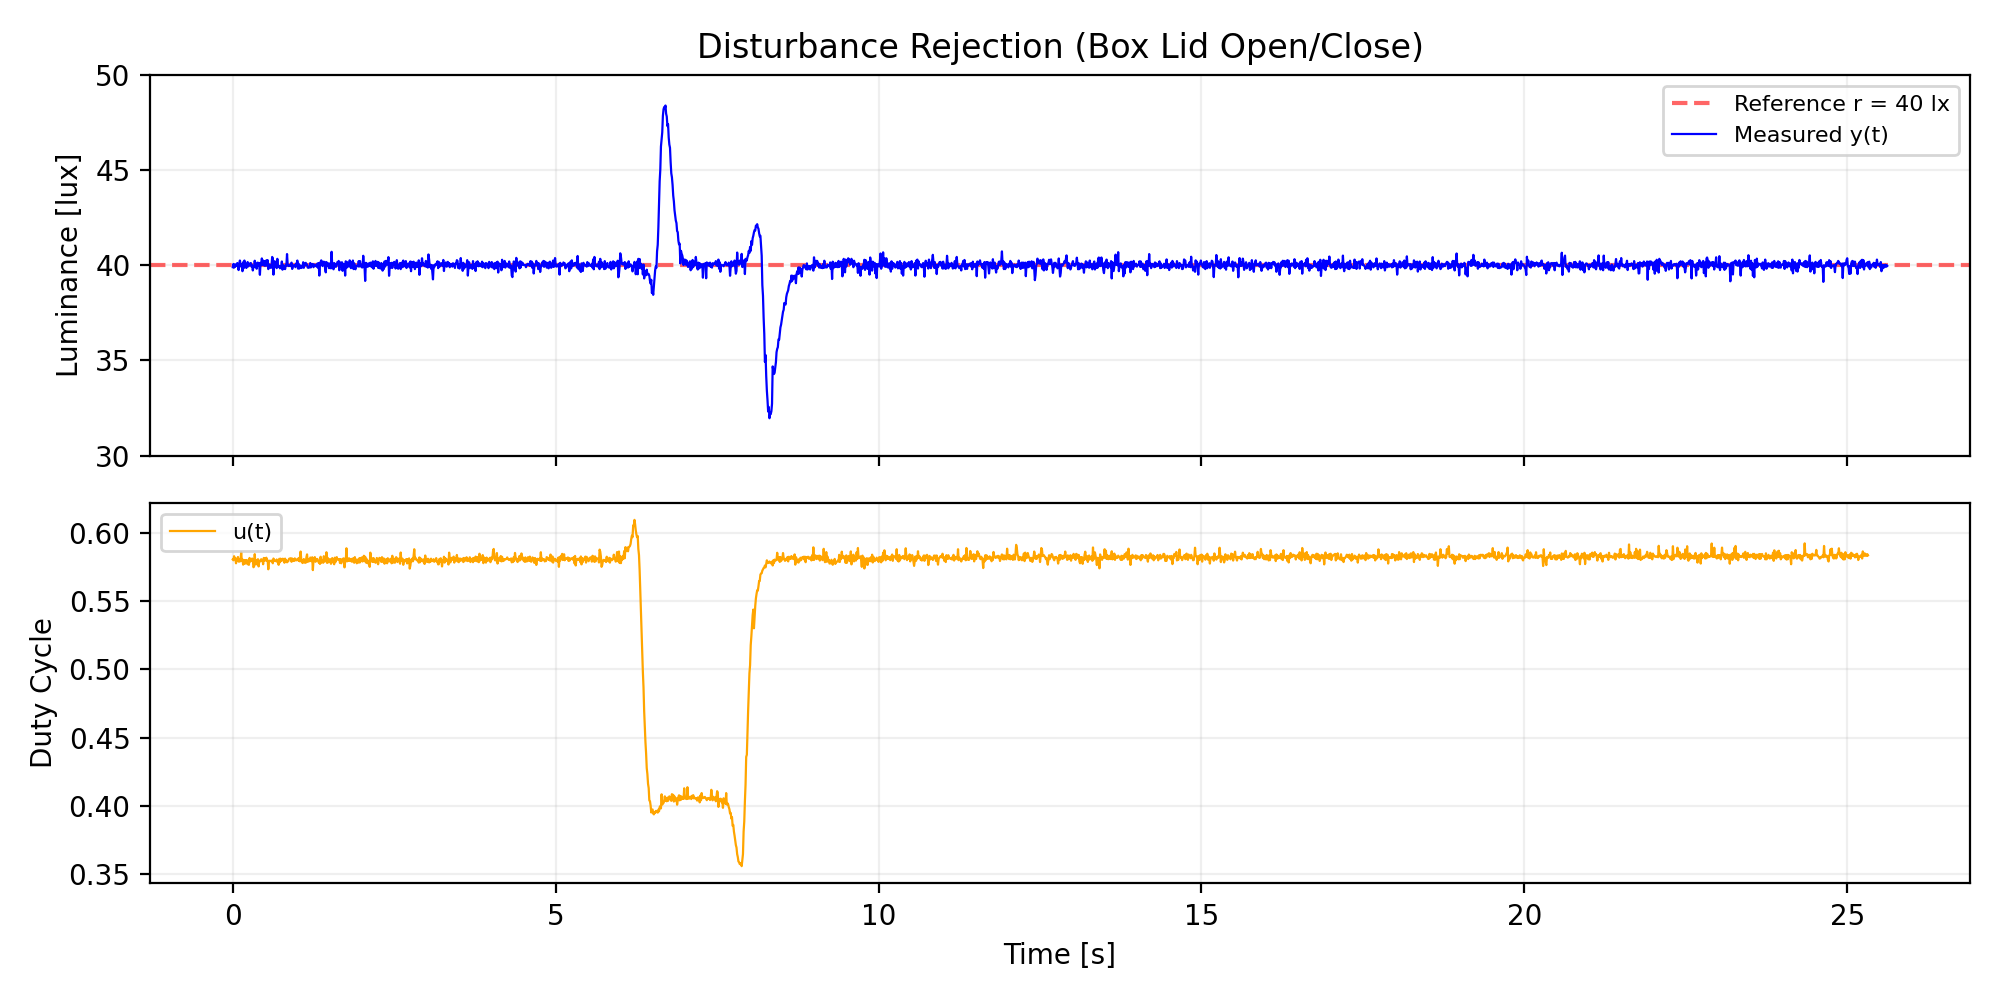
\includegraphics[width=\columnwidth]{figures/fig_disturbance.png}
  \caption{Disturbance rejection (box lid open/close).}
  \label{fig:disturbance}
\end{figure}

\subsection{Flicker and Jitter}

Fig.~\ref{fig:flicker} shows the duty cycle over \SI{30}{\second} at steady state: peak-to-peak variation is less than 0.02, corresponding to a flicker metric of $1.6 \times 10^{-4}$. Fig.~\ref{fig:jitter} confirms zero timing jitter: all 1031 measured inter-sample intervals are exactly \SI{10}{\milli\second}. Table~\ref{tab:metrics} summarises all steady-state metrics.

\begin{figure}[H]
  \centering
  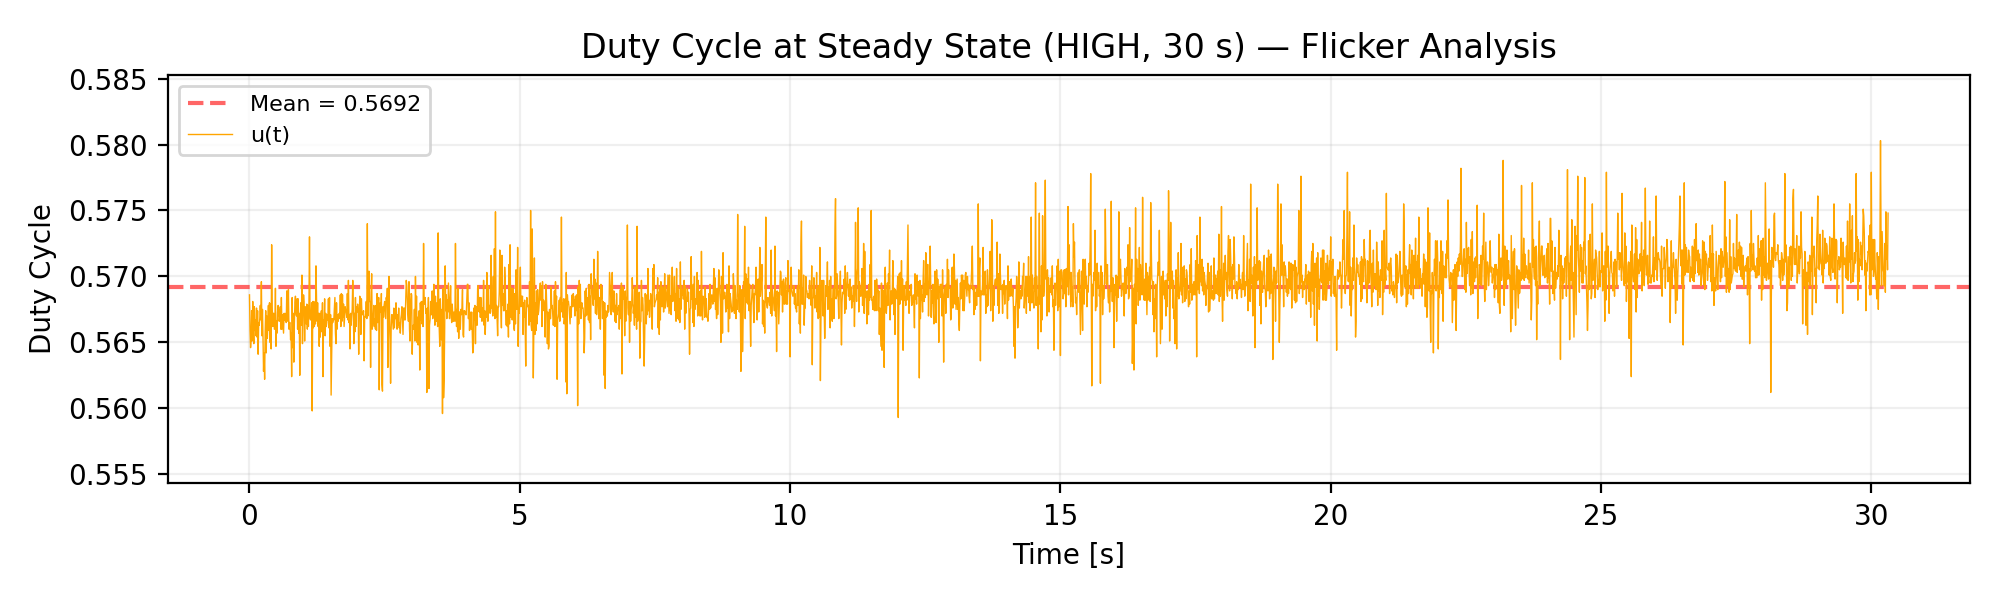
\includegraphics[width=\columnwidth]{figures/fig_flicker.png}
  \caption{Duty cycle at steady state (\SI{30}{\second}). Low flicker confirmed.}
  \label{fig:flicker}
\end{figure}

\begin{figure}[H]
  \centering
  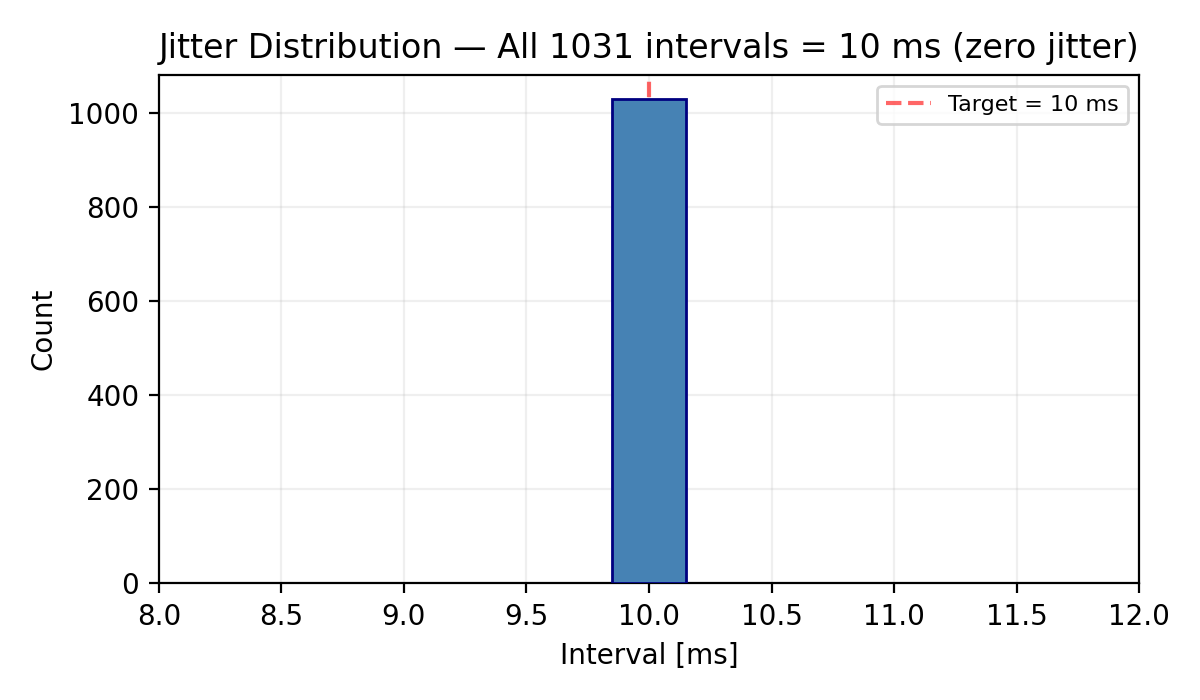
\includegraphics[width=0.75\columnwidth]{figures/fig_jitter.png}
  \caption{Jitter distribution. All 1031 intervals = \SI{10}{\milli\second} (zero jitter).}
  \label{fig:jitter}
\end{figure}

\begin{table}[H]
\centering
\caption{Steady-state performance metrics (HIGH, \SI{60}{\second}).}
\label{tab:metrics}
\small
\begin{tabular}{@{}lll@{}}
  \toprule
  Metric & Value & Unit \\
  \midrule
  Energy $E$              & $179.4$              & \si{\joule} \\
  Visibility error $V$    & $0.04$               & \si{\lux} \\
  Flicker $F$             & $1.6 \times 10^{-4}$ & -- \\
  Jitter (max)            & $0$                  & \si{\micro\second} \\
  Settling (H$\to$L / L$\to$H) & $0.43$ / $0.27$ & \si{\second} \\
  Overshoot               & $< 2.5$              & \% \\
  \bottomrule
\end{tabular}
\end{table}

\section{Serial Command Interface}

A serial protocol at 115200\,baud was implemented following the project specification~\cite{projectguide}. Table~\ref{tab:commands} lists the supported commands.

\begin{table}[H]
\centering
\caption{Serial command interface summary.}
\label{tab:commands}
\scriptsize
\setlength{\tabcolsep}{3pt}
\begin{tabular}{@{}lll@{}}
  \toprule
  \textbf{Command} & \textbf{Format} & \textbf{Description} \\
  \midrule
  \multicolumn{3}{@{}l}{\textit{Setters}} \\
  Set duty cycle    & \texttt{d <i> <val>}  & Direct PWM control \\
  Set reference     & \texttt{r <i> <val>}  & Illuminance target \\
  Set occupancy     & \texttt{o <i> <0|1>}  & Unocc./occupied \\
  Anti-windup       & \texttt{a <i> <0|1>}  & Toggle ON/OFF \\
  Feedback          & \texttt{k <i> <0|1>}  & Toggle ON/OFF \\
  \midrule
  \multicolumn{3}{@{}l}{\textit{Getters}} \\
  Get variable      & \texttt{g <x> <i>}    & \texttt{x}: d,r,l,o,a,k,x,p,t,e,v,f \\
  Last-min buffer   & \texttt{g b <l|d> <i>} & 6000 samples \\
  \midrule
  \multicolumn{3}{@{}l}{\textit{Streaming}} \\
  Start/stop        & \texttt{s/S <l|d> <i>} & Real-time lux/duty \\
  \midrule
  \multicolumn{3}{@{}l}{\textit{Controller}} \\
  Change params     & \texttt{c <k|i|b|t> <i> <val>} & $K_p$/$K_i$/$b_\mathrm{sp}$/$T_t$ \\
  Recalibrate       & \texttt{c r <i>}      & Measure $K_s$, $L_\mathrm{bg}$ \\
  \bottomrule
\end{tabular}
\end{table}

\section{Conclusions}

A PI controller without feedforward was shown to achieve sub-\SI{0.5}{\second} settling time with less than 2.5\% overshoot by avoiding abrupt duty-cycle transitions that trigger CdS LDR persistence. The back-calculation anti-windup and set-point weighting provide robust performance across operating conditions. The calibration routine and on-line parameter adjustment commands enable adaptation to different box geometries and luminaire placements. For the second project stage, the coupling gains from neighbouring luminaires will be incorporated into the control law, and the CAN-BUS communication layer will enable cooperative distributed control across multiple desks.

\begin{thebibliography}{9}
\bibitem{projectguide}
  A.~Bernardino \textit{et al.},
  \textit{Distributed Real-Time Control Systems --- Project Guide},
  IST, v1.0, 2025--2026.
\bibitem{ldr}
  Token Electronics,
  \textit{PGM CDS Photoresistors --- Light-Dependent Photoresistors for Sensor Applications},
  PGM5659D datasheet, 2010.
\bibitem{led}
  OptoSupply,
  \textit{10\,mm Bullet Pure White LED},
  OSW5DKA201A datasheet.
\end{thebibliography}

\end{document}
